\documentclass{article}
\usepackage[utf8]{inputenc}
\usepackage{amsmath}
\usepackage[a4paper,body={140mm,250mm}]{geometry}

\usepackage{graphicx} 
\usepackage{array} 
\usepackage{newtxtext,newtxmath}
\usepackage[varl]{inconsolata}

\begin{document}
\begin{titlepage}
  \begin{flushleft}\scshape
    Lund University\\
    Automatic Control\\[\smallskipamount]
    FRTN40 Project in automatic control\\
    Autumn 2018
  \end{flushleft}
  \vspace*{0pt plus 0.3fill}
  \begin{center}
    \huge \textbf{Autonomous Driving (F1tenth) }\\[4mm]     
    \large\textbf{Project Plan Group C}\\[5mm]
         Albert Anderberg\footnote{\texttt{albert.anderberg.477@student.lu.se}}\quad
         Josiah Wong\footnote{\texttt{jo7036wo-s@student.lu.se}}\quad
         Rebeca Homssi\footnote{\texttt{rebeca.homssi.322@student.lu.se}}
  \end{center}
\begin{center}
    Project Advisor: Martina Maggio
\end{center}
\vfill
\end{titlepage}        

\section{Project Purpose}
The goal of this project is to create a controller and a path planning model that can navigate the f1/tenth car through an unknown path keeping a certain distance to the wall and avoiding obstacles that can appear on the way based on feedback from the LIDAR sensor and the IMU. The aim is to develop the path planning model to be able to navigate the car to overtake another car. The work will be based on previous work that is available on the page http://f1tenth.org/.

\section{Equipments \& Material} \label{sec:equipment}
The two F1/tenth cars provided is already built together and complete. Therefore no new materials needs to be ordered but some plastic pieces on the car may need to be replaced. For example is the transparent vertical plastic separating the transparent top and the bottom of the car a little broken. If needed the piece will be 3D-printed.

\section{Modeling \& System Design}
The f1/10 car are built on the Nvidia Jetson TK1 development kit which runs Ubuntu and ROS. Since ROS is based around nodes and topics it is simple to divide the different computations into different nodes that will communicate with each other using different topics. This makes it possible to first decide what each node should do and which other nodes it should communicate with. Then the actual program for each node can be written independently of the other nodes.

As an example the sensors acts as two different nodes and the controller can subscribe to the topics they produce. A possible program structure can be seen in figure~\ref{fig:SystemDesign}. The software is divided between the development board on the car and a remote computer. The remote computer will run the software containing the user interface. The user interface could have different functions, for example mode switching, live plotting of measurement values and safety functions such as emergency stop. The development platform has the software that reads measurement data, calculates the control signal and communicates with the remote system.

\begin{figure} [h]
	\centering
 	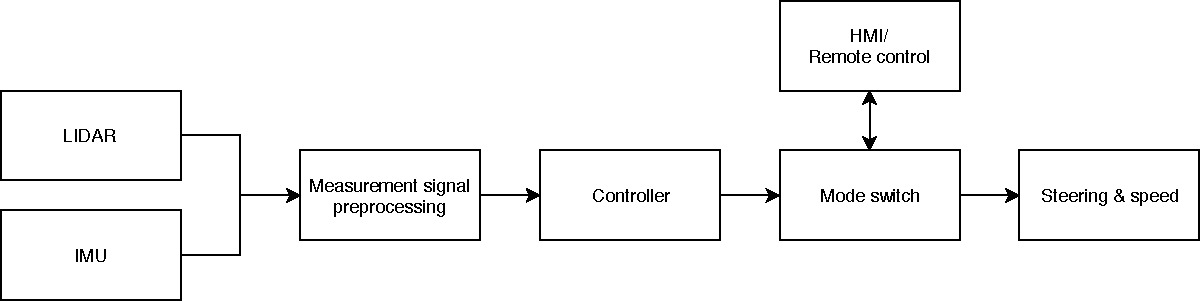
\includegraphics[width=0.85\textwidth]{figures/FRTN40-SystemDesign}
    \caption{The structure of the software.}
    \label{fig:SystemDesign}
\end{figure}


\section{Division of Labour} \label{sec:division}

The program we will develop basically consist of four nodes. One node that will process all the information from the LiDAR and therefore be able to detect obstacles in the way. When an obstacle is blocking the current path the node will signal this to the path planning node. The path planning node will then create a new path to avoid hitting the obstacle. The new path is sent over to the controller node. The controller node handles the PID controller in the car and therefore all the steering. The controller node will also communicate with the IMU node which collects and processes data of the speed and acceleration of the car. 

As mentioned before, the nodes is independent of each other and can only communicates through topics. This makes it easy to divide the work so each person can build up a node.




\section{Time Plan}
\subsection{Subtasks}
    \begin{itemize}
        \item Implement basic code to make the car driving on a straight path. \textbf{Estimated deadline}: 19/11
        \item Do some signal processing of the data from the LiDar sensor.  \textbf{Estimated deadline}: 19/11
        \item Research and planning of path planning model for avoid hitting an object. \textbf{Estimated deadline}: 19/11
        \item Implement the path planning model. \textbf{Estimated deadline}: 26/11    
        \item Test the path planing model. \textbf{Estimated deadline}: 3/12
        \item Upgrade the path planning model to also be able to build a path for when the object is moving.  \textbf{Estimated deadline}: 10/12
        \item Test the upgraded path planning model. \textbf{Estimated deadline}: 16/12
        
    \end{itemize}
    
\subsection{Important dates}
    \begin{itemize}
        \item 9/11 -  Hand in project plan.
        \item 19/11 - Feedback seminar 1 on the modeling and design.
        \item 5/12 - Report should be pushed to git to allow peer review by other groups.
        \item 10/12 - Feedback seminar 2 on the design and implementation.
        \item 17/12 - The whole process should be finished and ready for demonstration.
        \item 20/12 - A complete project report should be pushed to git and the supervisor notified.
        \item 10/1 - Project presentation and demonstration.
        \item 18/1 - A final revised report should be pushed to git and the supervisor notified.
    \end{itemize}

\subsection{Gantt Chart}
    We have formalized the time plan as a Gantt chart. The major tasks can be seen plotted in Figure~\ref{fig:gantt}.
    \begin{figure} [ht]
        \centering
        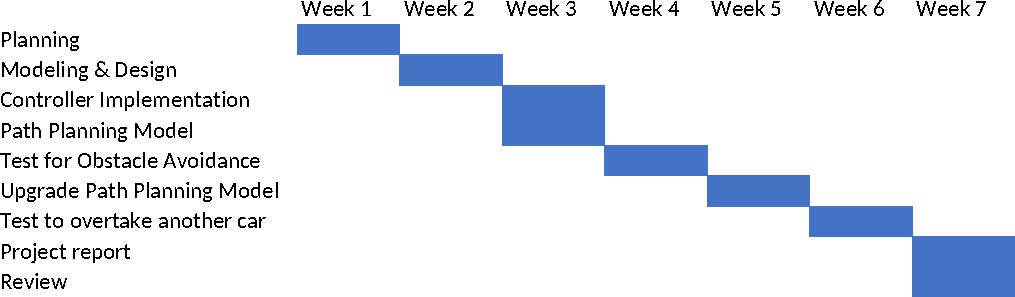
\includegraphics[width=0.95\textwidth]{figures/timePlan}
        \caption{The Gantt chart describing the work flow of our project.}
        \label{fig:gantt}
    \end{figure}

\end{document}
